\section{Pointer to Primitive Type Variables}
\label{sec:structs}
\begin{frame}<beamer>
    \frametitle{Outline}
    \tableofcontents[currentsection]
\end{frame}

\begin{frame}
	\begin{figure}
		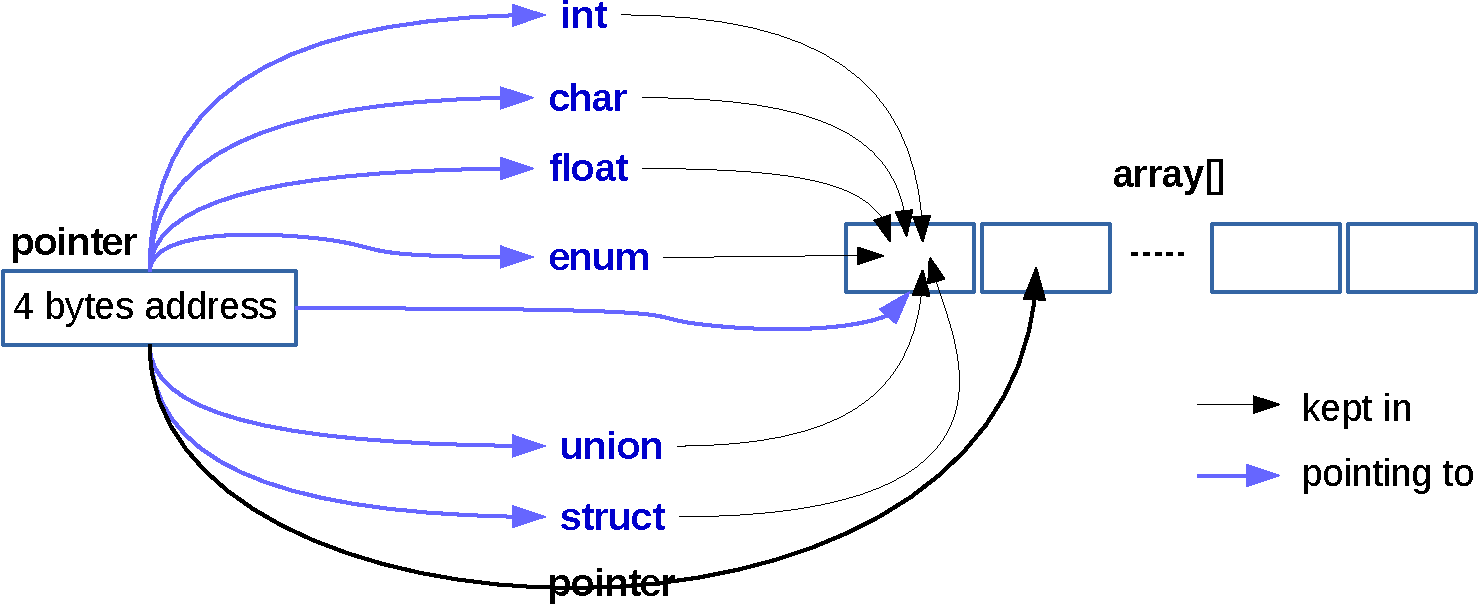
\includegraphics[width=0.92\linewidth]{figs/pt_type_demo.pdf}
	\end{figure}
	\begin{itemize}
		\item {Pointer essentially is the address of a variable}
		\item {Any types of variable has an address}
		\item {Array has address too}
		\item {It is allowed to have pointer array (array of addresses)}
	\end{itemize}
\end{frame}

\begin{frame}[fragile]{Grammar for pointer definition}
\begin{center}
	\Large{
	  \textcolor{blue}{dataType} \textbf{*}\textcolor{red}{pointVariableName}
	}
\end{center}
\begin{itemize}
	\item {Pointer is a variable too}
	\item {A variable keeps address of other variable(s)}
	\item {``*'' followed by variable name of the pointer}
\end{itemize}
\begin{lstlisting}[xleftmargin=0.08\linewidth, linewidth=0.9\linewidth]
int main()
{
   int *pt; //pointer points to an integer variable
}
\end{lstlisting}
\end{frame}

\begin{frame}[fragile]{Pointer initialization}
\begin{itemize}
	\item {Pointer is a variable too}
	\item {A variable keeps address of other variable(s)}
	\item {``*'' followed by variable name of the pointer}
\end{itemize}
\begin{lstlisting}[xleftmargin=0.01\linewidth, linewidth=0.99\linewidth]
#include <string.h>
#include <stdio.h>
int main()
{
   short *pt = NULL;//points to an integer variable
   float a = 3.1;
   float *fpt = &a;
   printf("Size of pt: %d\n", sizeof(pt));
   printf("Size of fpt: %d\n", sizeof(fpt));
   printf("Size of short: %d\n", sizeof(short));
}
\end{lstlisting}
\vspace{-0.15in}
\begin{itemize}
	\item {``\&'' is an operator (\textcolor{green}{something new!})}
	\item {``\&a'' extracts the address of variable \textbf{a}}
	\item {Address of variable \textbf{a} (4 bytes number) is then assigned to ``fpt''}
\end{itemize}
\end{frame}

\begin{frame}[fragile]{Pointer in its nature}
\vspace{-0.15in}
\begin{columns}
\begin{column}{0.45\linewidth}
\begin{lstlisting}
#include <string.h>
#include <stdio.h>
int main()
{
   int a = 6;
   int *b = &a;
   ....
\end{lstlisting}
\end{column}
\begin{column}{0.5\linewidth}
\begin{figure}
\begin{center}
	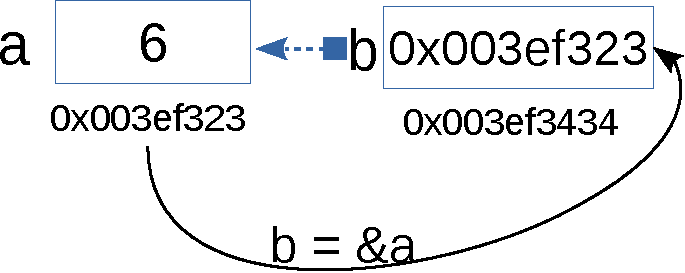
\includegraphics[width=0.8\linewidth]{figs/pointer.pdf}
\end{center}
\end{figure}
\end{column}
\end{columns}
\vspace{-0.15in}
\begin{itemize}
	\item {``\&a'' extracts the address of variable \textbf{a}}
	\item {Address of variable \textbf{a} (4 bytes number) is then assigned to ``fpt''}
\end{itemize}
\end{frame}

\begin{frame}[fragile]{Visit variable by its pointer (1)}
\vspace{-0.15in}
\begin{columns}
\begin{column}{0.56\linewidth}
\begin{lstlisting}[xleftmargin=0.05\linewidth, linewidth=0.95\linewidth]
#include <string.h>
#include <stdio.h>
int main()
{
   short a = 4;
   short *pa= &a;
   float b = 3.1;
   float *pb = &b;
   printf("a = %d\n", a);
   printf("b = %f\n", b);
   printf("*pa = %d\n", *pa);
   printf("*pb = %f\n", *pb);
   printf("pa = %ld\n", pa);
   printf("pb = %ld\n", pb);
   return 0;
}
\end{lstlisting}
\end{column}
\begin{column}{0.41\linewidth}
[Output:]
\begin{lstlisting}
??
??
??
??
??
??
\end{lstlisting}
\end{column}
\end{columns}
\vspace{-0.1in}
\begin{itemize}
	\item {``*pa'' takes the value from the address kept by pa}
\end{itemize}
\end{frame}


\begin{frame}[fragile]{Visit variable by its pointer (2)}
\vspace{-0.15in}
\begin{columns}
\begin{column}{0.56\linewidth}
\begin{lstlisting}[xleftmargin=0.02\linewidth, linewidth=0.98\linewidth]
#include <string.h>
#include <stdio.h>
int main()
{
   short a = 4;
   short *pa= &a;
   float b = 3.1;
   float *pb = &b;
   printf("a = %d\n", a);
   printf("b = %f\n", b);
   printf("*pa = %d\n", *pa);
   printf("*pb = %f\n", *pb);
   printf("pa = %ld\n", pa);
   printf("pb = %ld\n", pb);
   return 0;
}
\end{lstlisting}
\end{column}
\begin{column}{0.41\linewidth}
[Output:]
\begin{lstlisting}
4
3.1
4
3.1
0439082323
0439082336
\end{lstlisting}
\end{column}
\end{columns}
\vspace{-0.1in}
\begin{itemize}
	\item {``*pa'' takes the value from the address kept by pa}
\end{itemize}
\end{frame}

\begin{frame}[fragile]{Visit variable by its pointer (3)}
\vspace{-0.15in}
\begin{columns}
\begin{column}{0.56\linewidth}
\begin{lstlisting}[xleftmargin=0.02\linewidth, linewidth=0.98\linewidth]
#include <string.h>
#include <stdio.h>
int main()
{
   float a = 4.5;
   float b = 3.1;
   float *p = &a;
   printf("p = %x\n", p);
   p = &b;
   printf("*p = %f\n", *p);
   printf("p = %x\n", p);
   *p = 7.2;
   p  = &a;
   *p = 5 .3;
   printf("a = %f\n", a);
   printf("b = %f\n", b);
   return 0;
}
\end{lstlisting}
\end{column}
\begin{column}{0.41\linewidth}
[Output:]
\begin{lstlisting}
?
?
?
?
?
\end{lstlisting}
\end{column}
\end{columns}
\vspace{-0.1in}
\begin{itemize}
	\item {``*pa'' takes the value from the address kept by pa}
\end{itemize}
\end{frame}

\begin{frame}[fragile]{Revisit: swap values of \textit{a} and \textit{b} (1)}
\vspace{-0.25in}
\begin{columns}
\begin{column}{0.47\linewidth}
\begin{lstlisting}
#include <stdio.h>
void swap(int a, int b)
{
   int tmp = a;
   a = b;
   b = tmp;
   return ;
}
int main()
{
  int a = 3; 
  int b = 5;
  printf("a=%d,b=%d\n",a,b);
  swap(a, b);
  printf("a=%d,b=%d\n",a,b);
  return 0;
}
\end{lstlisting}
\end{column}
\begin{column}{0.47\linewidth}
\begin{lstlisting}[xleftmargin=0.005\linewidth]
#include <stdio.h>
int a, b;
void swap()
{
  int tmp = a;
  a = b;
  b = tmp;
  return ;
}
int main()
{
  a = 3; 
  b = 5;
  printf("a=%d,b=%d\n",a,b);
  swap(a, b);
  printf("a=%d,b=%d\n",a,b);
  return 0;
}
\end{lstlisting}
\end{column}
\end{columns}
\end{frame}

\begin{frame}[fragile]{Revisit: swap values of \textit{a} and \textit{b} (2)}
\vspace{-0.25in}
\begin{columns}
\begin{column}{0.47\linewidth}
\begin{lstlisting}
#include <stdio.h>
void swap(int a, int b)
{
   int tmp = a;
   a = b;
   b = tmp;
   return ;
}
int main()
{
  int a = 3; 
  int b = 5;
  printf("a=%d,b=%d\n",a,b);
  swap(a, b);
  printf("a=%d,b=%d\n",a,b);
  return 0;
}
\end{lstlisting}
\end{column}
\begin{column}{0.47\linewidth}
\begin{lstlisting}[xleftmargin=0.005\linewidth]
#include <stdio.h>
void swap(int *a, int *b)
{
   int tmp = *a;
   *a = *b;
   *b = tmp;
   return ;
}
int main()
{
  int a = 3; 
  int b = 5;
  printf("a=%d,b=%d\n",a,b);
  swap(&a, &b);
  printf("a=%d,b=%d\n",a,b);
  return 0;
}
\end{lstlisting}
\end{column}
\end{columns}
\end{frame}

\begin{frame}[fragile]{Revisit: swap values of \textit{a} and \textit{b} (3)}
\begin{figure}
	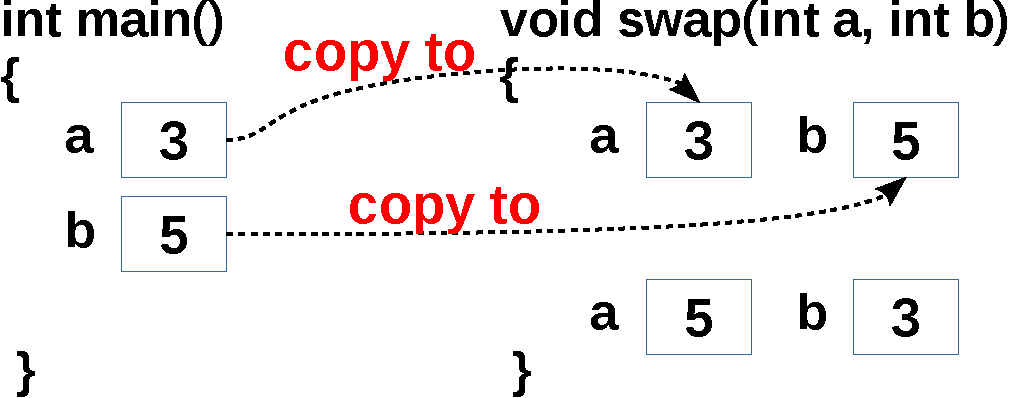
\includegraphics[width=0.55\linewidth]{figs/swap1.pdf}
	\caption{What happens for swap(int a, int b).}
\end{figure}

\begin{figure}
	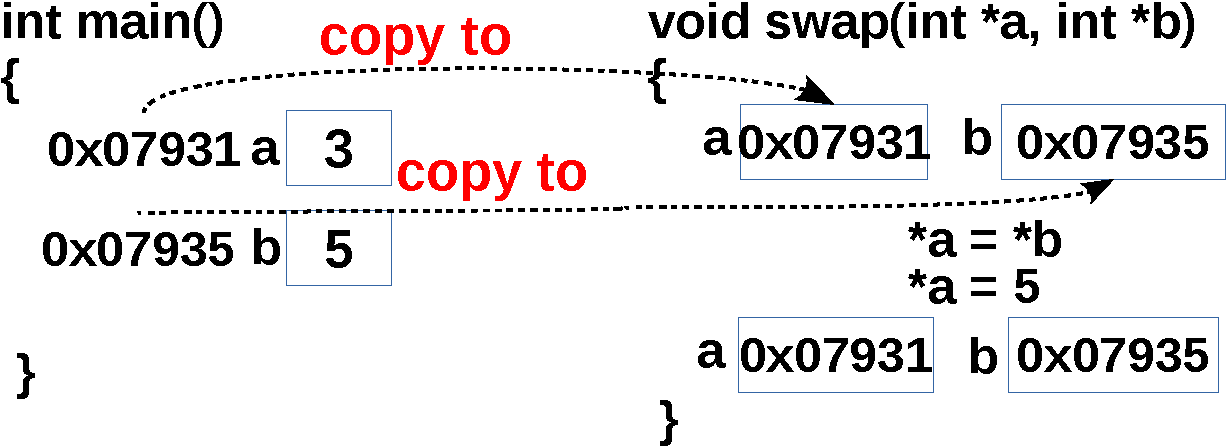
\includegraphics[width=0.62\linewidth]{figs/swap2.pdf}
	\caption{What happens for swap(int *a, int *b).}
\end{figure}
\end{frame}


\begin{frame}[fragile]{Revisit: swap values of \textit{a} and \textit{b} (4)}
\vspace{-0.25in}
\begin{columns}
\begin{column}{0.47\linewidth}
\begin{lstlisting}
#include <stdio.h>
void swap(int *a, int *b)
{
   int tmp = *a;
   *a = *b;
   *b = tmp;
   return ;
}
int main()
{
  int a = 3; 
  int b = 5;
  printf("a=%d,b=%d\n",a,b);
  swap(&a, &b);
  printf("a=%d,b=%d\n",a,b);
  return 0;
}
\end{lstlisting}
\end{column}
\begin{column}{0.47\linewidth}
\begin{lstlisting}[xleftmargin=0.005\linewidth]
#include <stdio.h>
void swap(adr a, adr b)
{
   int tmp = *a;
   *a = *b;
   *b = tmp;
   return ;
}
int main()
{
  int a = 3; 
  int b = 5;
  printf("a=%d,b=%d\n",a,b);
  swap(&a, &b);
  printf("a=%d,b=%d\n",a,b);
  return 0;
}
\end{lstlisting}
\end{column}
\end{columns}
\vspace{-0.1in}
\begin{itemize}
	\item {Given \textcolor{blue}{adr} is an address type}
\end{itemize}
\end{frame}

\begin{frame}[fragile]{Summary over Pointer to Variables (1)}
\vspace{-0.15in}
\begin{itemize}
	\item {Pointer is a variable or constant}
    \item {It keeps the address of a variable}
    \item {One is allowed to do operation on a variable by its address}
\end{itemize}
\begin{columns}
\begin{column}{0.4\linewidth}
\begin{lstlisting}
#include <stdio.h>
int main()
{
   int a = 3, *p;
   int b = 1;
   p = &a;
   printf("a=%d\n", *p);
   p = &b;
   printf("b=%d\n", *p);
}
\end{lstlisting}
\end{column}
\begin{column}{0.45\linewidth}
\begin{lstlisting}
void incr(int *a)
{
   *a = *a + 1;
}
int main()
{
 int a = 4, *b = &a;
 printf("%d\n", *b);
 incr(&a);
 printf("%d\n", a);
 printf("%d\n", *b);
 return 0;
}
\end{lstlisting}
\end{column}
\end{columns}
\end{frame}

\begin{frame}[fragile]{Summary over Pointer to Variables (2)}
\vspace{-0.15in}
\begin{itemize}
	\item {Pointer is a variable or constant}
    \item {It keeps the address of a variable}
    \item {One is allowed to do operation on a variable by its address}
\end{itemize}
\begin{columns}
\begin{column}{0.4\linewidth}
\begin{lstlisting}
#include <stdio.h>
int main()
{
   int a = 3, *p;
   int b = 1;
   *p = a;
   p  = b;
   p  = &c;
}
\end{lstlisting}
\end{column}
\begin{column}{0.45\linewidth}
\begin{lstlisting}
#include <stdio.h>
int main()
{
   int a = 3, *p;
   int b = 1;
   float c = 2.2;
   p   = &a;
   printf("%d", *p);
   *p  = b;
   printf("%d", *p);
   printf("%d", a);
}
\end{lstlisting}
\end{column}
\end{columns}
\end{frame}

\begin{frame}[fragile]{Summary over Pointer to Variables (3)}
\vspace{-0.15in}
\begin{columns}
\begin{column}{0.4\linewidth}
\begin{lstlisting}
void incr(int *a)
{
   *a = *a + 1;
}
int main()
{
 int a = 4, *b = &a;
 printf("%d\n", *b);
 incr(&a);
 printf("%d\n", a);
 printf("%d\n", *b);
 return 0;
}
\end{lstlisting}
\end{column}
\begin{column}{0.45\linewidth}
\begin{lstlisting}
void incr(int *a)
{
   a = a + 4;
}
int main()
{
 int a = 4, *b = &a;
 printf("%d\n", *b);
 incr(&a);
 printf("%d\n", a);
 printf("%d\n", *b);
 return 0;
}
\end{lstlisting}
\end{column}
\end{columns}
\begin{itemize}
	\item {`incr(int* a)' on the right, increases the address number of \textbf{a}}
    \item {It points to \textcolor{red}{another memory cell}}
    \item {\textbf{a} inside `incr(int *a)' is a local variable}
    \item {It has no effect on input variable}
\end{itemize}
\end{frame}

\begin{frame}[fragile]{Explained}
\vspace{-0.15in}
\begin{columns}
\begin{column}{0.4\linewidth}
\begin{lstlisting}
void incr(adr a)
{
   *a = *a + 1;
}
int main()
{
 int a = 4, *b = &a;
 printf("%d\n", *b);
 incr(&a);
 printf("%d\n", a);
 printf("%d\n", *b);
 return 0;
}
\end{lstlisting}
\end{column}
\begin{column}{0.45\linewidth}
\begin{lstlisting}
void incr(adr a)
{
   a = a + 4;
}
int main()
{
 int a = 4, *b = &a;
 printf("%d\n", *b);
 incr(&a);
 printf("%d\n", a);
 printf("%d\n", *b);
 return 0;
}
\end{lstlisting}
\end{column}
\end{columns}
\begin{itemize}
	\item {Given \textcolor{blue}{adr} is an address type}
    \item {Keep the principle that parameter ``\textcolor{red}{transfer by value}'' in C}
    \item {\textbf{a} inside `incr(\textcolor{blue}{adr} a)' is a local variable}
    \item {It has no effect on input variable}
\end{itemize}
\end{frame}

\begin{frame}[fragile]{A Revisit about ``scanf($\cdot$,$\cdot$)''}
\vspace{-0.10in}
\begin{lstlisting}[xleftmargin=0.08\linewidth, linewidth=0.9\linewidth]
int main()
{
  int a = 0;
  printf("Input value for a: ");
  scanf("%d", &a); //<-- pay attention to here
  return 0;
}
\end{lstlisting}
\vspace{-0.15in}
\begin{itemize}
	\item {Now we should be clear why we put ``\&'' before \textbf{a}}
	\item {By this way, we tell \textbf{scanf}($\cdot$) to put the user input value to which memory address}
	\item {Is it possible if we do something as following?}
\end{itemize}
\begin{lstlisting}[xleftmargin=0.01\linewidth, linewidth=0.99\linewidth]
int main()
{
  int a = 0;
  printf("Input value for a: ");
  scanf("%d", a); //<--ask yourself whether this is valid??
  return 0;
}
\end{lstlisting}
\end{frame}